\section{Demo Applications}
\label{subsec: Demo Applications}

This project provides some \textbf{demo applications} with practical examples which show the main \textbf{FreeRTOS} functionalities. \textbf{QEMU} was used for virtualizing the \textbf{ARM Cortex-M3 processor}, i.e., the target architecture, and for testing all the \textbf{demo applications}. 

\subsection{Background}
\label{subsec: Background}
The main FreeRTOS functions are contained in the following files:
\begin{itemize}
    \item \texttt{task.c}
    \item \texttt{queue.c}
    \item \texttt{list.c}
\end{itemize}

Before running the selected demo application, there is the need to build the project (as already seen in \ref{subsec: Building the Demo}) in order to compile the \textbf{FreeRTOS source code} and link it with our \textbf{demo application}.

Moreover, the processor requires some additional \textbf{RTOS code} for the target architecture.
This part is located in the \texttt{FreeRTOS/FreeRTOS/Source/portable} \texttt{/[compiler]/[architecture]} directory.
In our case the \textit{compiler} is \textbf{GCC} (\textbf{GNU Compliler Collection}) and the \textit{architecture} is \textbf{ARM\_CM3} which refers to the \textbf{ARM Cortex-M3 processor}.

Furthermore, the files which handle the \textbf{memory management} are located in the 
\\ \texttt{FreeRTOS/FreeRTOS/Source}\texttt{/portable/MemMang} and are called \texttt{heap\_x.c}. Typically \texttt{heap\_4.c} is used. In our project, a revised version of \texttt{heap\_4.c} will be proposed and tested in the section \ref{sec: Memory Management}.

Another important file is the \texttt{FreeRTOSConfig.h} header file which contains all the configurations options for the \textbf{Real Time OS}.

\subsection{Intro to the demo applications}
The demo applications are divided into two sections in order to provide a comprehensive overview about two of the main macro-themes of FreeRTOS distribution:
\begin{itemize}
    \item \textbf{Task Management}
    \item \textbf{Queue and Tasks' Synchronization}
\end{itemize}
In this project, each single demo application can be selected by properly setting the \texttt{mainCREATE\_SIMPLE\_DEMO} value in the \texttt{main.c} file. 

\subsubsection{Task Management} 
\label{subsubsec: Task Management}
This subsection provides three different demo applications:
\begin{enumerate}
    \item \texttt{mainCREATE\_SIMPLE\_DEMO = 1} selects the \texttt{main\_three\_tasks\_CRUDE.c} demo application.
    \item \texttt{mainCREATE\_SIMPLE\_DEMO = 2} selects the \texttt{main\_three\_tasks.c} demo application.
    \item \texttt{mainCREATE\_SIMPLE\_DEMO = 3} selects the \texttt{main\_priority.c} demo application.
\end{enumerate}
Each of them aims to let the reader understanding:
\begin{itemize}
    \item how to implement a task, create one or more instances of a task.
    \item how FreeRTOS allocates processing time to each task.
    \item how FreeRTOS scheduler works.
    \item how the relative priority of each task affects its behaviour.
\end{itemize}

\paragraph{Simple Example with CRUDE DELAY.}  
\label{par: Simple Example with CRUDE DELAY}
The \texttt{main\_three\_tasks\_CRUDE.c} application is a simple example which shows the main \textbf{FreeRTOS API functions} for \textbf{creating}, \textbf{developing} and \textbf{managing tasks} in an embedded system.
The application simply consists of \textbf{three tasks}. All of them have the same priority and each one implements the same function which \textbf{prints a message} and enters in a loop with the unique functionality to delay the task (a \textbf{CRUDE DELAY}, i.e. which does not move the task in the \textit{waiting list}).

The general behaviour of the three tasks changes by modifying the scheduler configurations in the \texttt{FreeRTOSConfig.h} file. Totally there are three possibilities:
\begin{itemize}
    \item by setting the \texttt{configUSE\_PREEMPTION} and \texttt{configUSE\_TIME\_SLICING}'s values respectively to \texttt{1} and \texttt{0}, the scheduler will be \textbf{preemptive}, \textbf{priority-based} with \textbf{no time slicing} (i.e., \textbf{ROUND ROBIN DISABLED}). With this configuration, when a task with higher priority enters in the ready state preempts the running task (with lower priority). Tasks with the same priority do not share \textbf{CPU time} (i.e., no round robin behaviour).  \\
    Considering our demo application, since all the \textbf{three tasks} have the \textbf{same priority}, the \textbf{first one} that enters in the running state, takes precedence and \textbf{continues to run}.
    \item by setting the \texttt{configUSE\_PREEMPTION} and \texttt{configUSE\_TIME\_SLICING}'s values respectively to \texttt{1} and \texttt{1}, the scheduler will be \textbf{preemptive}, \textbf{priority-based} with \textbf{time slicing enabled} (i.e., \textbf{ROUND ROBIN-LIKE}). With this configuration, tasks with higher priority preempts tasks with lower one. When one or more tasks have the same priority of the running one, they share \textbf{CPU time} by alternating each other when a time slice occurs. \\
    Considering our demo application, the three tasks \textbf{alternate each other} in an unpredictable way.
    \item by setting the \texttt{configUSE\_PREEMPTION} and \texttt{configUSE\_TIME\_SLICING}'s values respectively to \texttt{0} and \texttt{x}, the scheduler will be \textbf{NOT preemptive} and \textbf{priority-based}. This means that context switching happens only when the running task explicitly moves to a \textbf{NOT RUNNING STATE}
    (suspended, blocked, or ended).\\
    Considering our demo application, since all the \textbf{three tasks} have the \textbf{same priority}, the first one that enters in the \textbf{running state}, continues to run.
\end{itemize}

\begin{figure}[H]
    \centering
    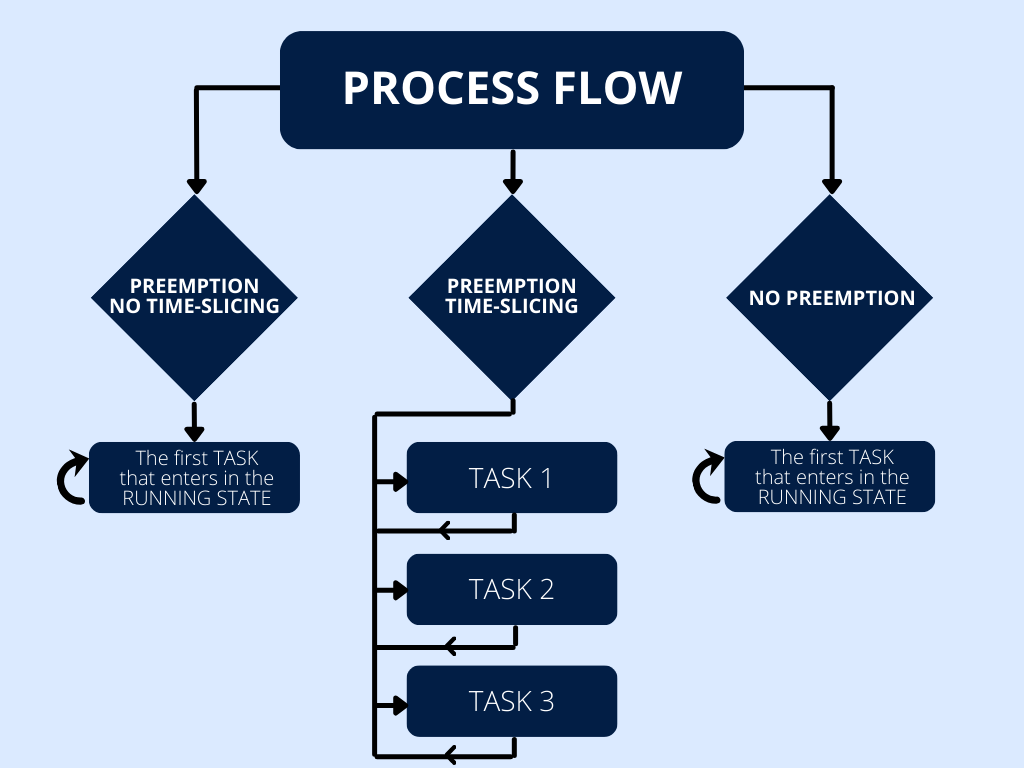
\includegraphics[width=0.5\textwidth]{img/three_tasks_CRUDE.png}
    \caption{Process Flow - main\_three\_tasks\_CRUDE.c}
    \label{fig:Process Flow - CRUDE DELAY}
\end{figure}


\paragraph{Example with DELAY/SLEEP FUNCTION.} 
\label{par: Simple Example with DELAY/SLEEP FUNCTION} 
The \texttt{main\_three\_tasks.c} application is a revised version of the previous one. The unique difference consists in the \textbf{implementation of the delay}. In this case the \textbf{API function} \texttt{vTaskDelayUntil()} offered by \textbf{FreeRTOS} is used to delay the task. This function just moves the task in the \textbf{blocked state}, making room for tasks in the \textbf{ready state}

Considering our demo application, the three tasks \textbf{alternate each other} independently from the \textbf{scheduler configuration}.

\begin{figure}[H]
    \centering
    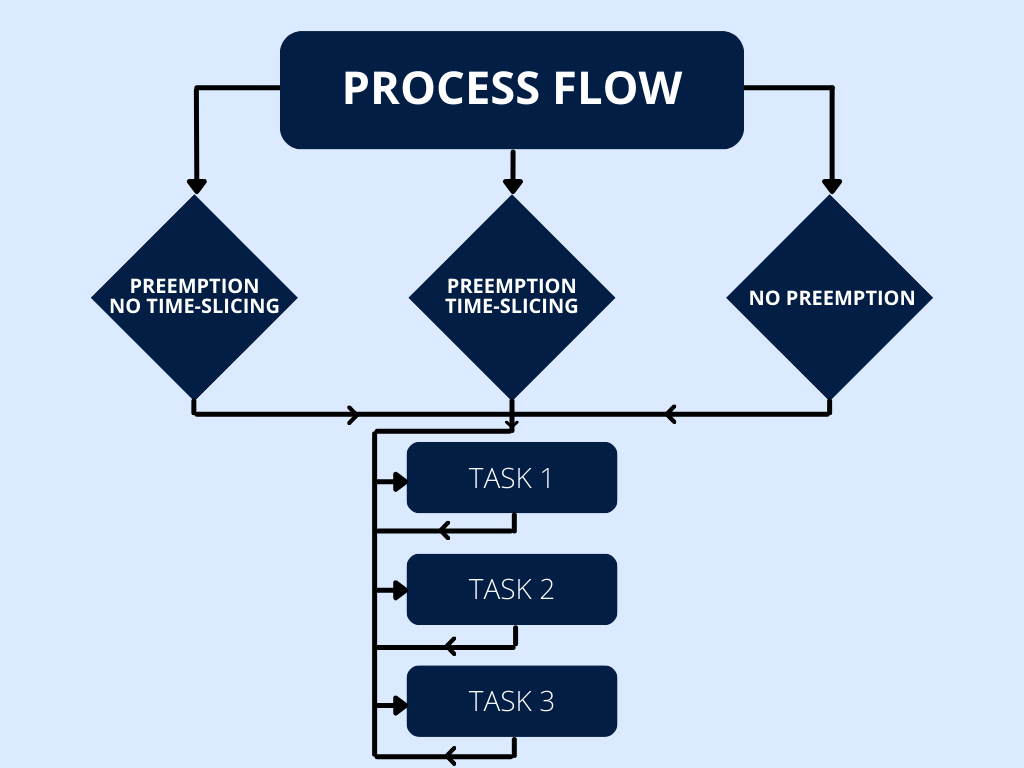
\includegraphics[width=0.5\textwidth]{img/three_tasks.png}
    \caption{Process Flow - main\_three\_tasks.c}
    \label{fig:Process Flow - vTaskDelayUntil}
\end{figure}

\paragraph{Example with Dynamic Priority.} 
\label{par: Simple Example with Dynamic Priority}
The \texttt{main\_priority.c} application is a more advanced example which aims to show how \textbf{FreeRTOS scheduler} works by analysing the behaviour of two tasks where one of them has dynamic priority.
The demo application consists of two tasks:
\begin{itemize}
    \item the \textbf{TASK 2} with lower priority (PRIORITY = 1), which creates the second task \textbf{TASK 1} (at the beginning with PRIORITY = 2), then enters in an infinite loop wherein it prints a message.
    \item the \textbf{TAKS 1} which continously changes its priority, first making it equal to \textbf{TASK 2}'s one, then increasing it again and so on...
\end{itemize}
\textbf{BOTH} the tasks implement a \textbf{CRUDE DELAY} with a for which consumes \textbf{CPU time} (i.e., the tasks are not moved into the waiting list).

The general behaviour of the three tasks changes by modifying the scheduler configurations:
\begin{itemize}
    \item \texttt{configUSE\_PREEMPTION = 1} and \texttt{configUSE\_TIME\_SLICING = 0} $\rightarrow$ the scheduler will be \textbf{preemptive}, \textbf{priority-based} with \textbf{no time slicing} (i.e., ROUND ROBIN DISABLED). In this case, \textbf{TASK 2} creates \textbf{TASK 1} which preempts \textbf{TASK 2} and continues to run.
    \item \texttt{configUSE\_PREEMPTION = 1} and \texttt{configUSE\_TIME\_SLICING = 1} $\rightarrow$ the scheduler will be \textbf{preemptive}, \textbf{priority-based} with \textbf{time slicing enabled} (i.e., ROUND ROBIN-LIKE). 
    In this case, \textbf{TASK 2} creates \textbf{TASK 1} which preempts \textbf{TASK 2}. When \textbf{TASK 1} decreases its priority, the two tasks alternate each other. At a certain point \textbf{TASK 1} increases again its priority continuing to run, and the same cycle will be repeated indefinitely.
    \item \texttt{configUSE\_PREEMPTION = 0} and \texttt{configUSE\_TIME\_SLICING = x} $\rightarrow$ the scheduler will be \textbf{NOT preemptive} and \textbf{priority-based}. 
    In this case, \textbf{TASK 2} creates \textbf{TASK 1} which \textbf{cannot} preempt \textbf{TASK 2} which continues to run indefinitely.
\end{itemize}

\begin{figure}[H]
    \centering
    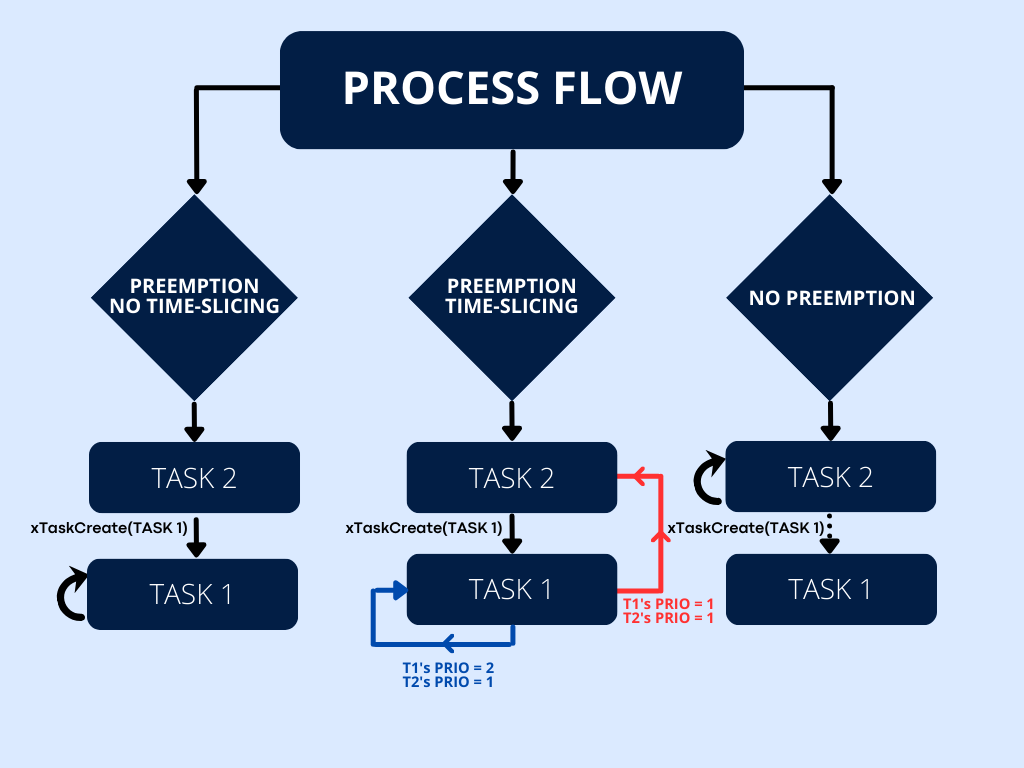
\includegraphics[width=0.5\textwidth]{img/dynamic_priority.png}
    \caption{Process Flow - main\_priority.c}
    \label{fig:Process Flow - Dynamic Priority}
\end{figure}

\subsubsection{Queue and Tasks' Synchronization}
\label{subsubsec: Queue and Tasks' Synchronization}

This subsection provides three different demo applications:
\begin{enumerate}
    \item \texttt{mainCREATE\_SIMPLE\_DEMO = 4} selects the \texttt{main\_queue.c} demo application.
    \item \texttt{mainCREATE\_SIMPLE\_DEMO = 5} selects the \texttt{main\_semaphore.c} demo application.
    \item \texttt{mainCREATE\_SIMPLE\_DEMO = 6} selects the \texttt{main\_semaphore2.c} demo application.
\end{enumerate}
Each of them aims to let the reader understanding:
\begin{itemize}
    \item how to use queues for task-to-task communication. 
    \item how use queues and semaphores for tasks'synchronization.
\end{itemize}

\paragraph{Simple Queue Example}. 
\label{par: Simple Queue Example}
This demo application shows the main \textbf{FreeRTOS API} functions for \textbf{Queue Management}. \textbf{Queues} provide \textbf{Task-to-Task} communication mechanism.
The \texttt{main\_queue} creates \textit{four tasks}:
\begin{itemize}
    \item three \textbf{PRODUCERS} which send items in the queue;
    \item one \textbf{CONSUMER} which reads from the queue.
\end{itemize}
The \textbf{CONSUMER} has the highest priority, the three \textbf{PRODUCERS} have the same priority.

When the scheduler starts the \textbf{CONSUMER} task tries to read from the queue which is empty. The \textbf{CONSUMER} task will block for \texttt{100 ms} waiting for data to be available. At this point one of the \textbf{PRODUCERS} will send data to the queue, unblocking the \textbf{CONSUMER} which will read the data from the queue. The \textbf{CONSUMER} task will then block again waiting for data and the cycle will continue. In this way the \textbf{PRODUCERS} will synchronize with the \textbf{CONSUMER} by just leveraging the \textbf{FreeRTOS queue implementation}.

Sometimes if the \texttt{100 ms} elapses while the queue is still empty, the \textbf{CONSUMER} task will print an \textbf{error message}. Moreover, each task contains a \textbf{CRUDE DELAY} implementation for \textbf{demonstration purposes}.
The general behaviour is depicted in the following diagram:

\begin{figure}[H]
    \centering
    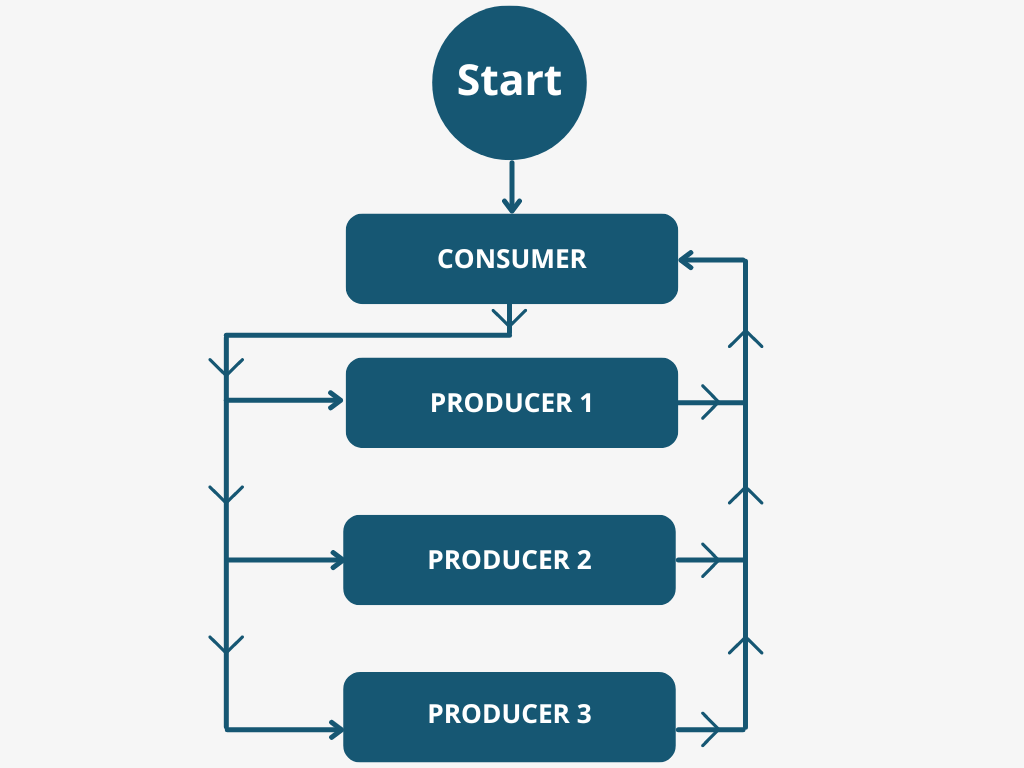
\includegraphics[width=0.5\textwidth]{img/main_queue.png}
    \caption{Precedence Diagram - Queue}
    \label{fig:Precedence Diagram - Queue}
\end{figure}


\paragraph{Queue and Semaphores: Example 1}.
\label{par:Queue and Semaphores 1}
This demo application shows the main \textbf{FreeRTOS} API functions for \textbf{Tasks' Synchronization} using \textbf{semaphores}. \textbf{Semaphores} are objects used to send interrupts for unblocking tasks. This results in tasks synchronization with interrupts.
The \texttt{main\_semaphore} creates the \textbf{queue}, the \textbf{semaphores} and \textbf{four tasks} with the \textbf{SAME priority}:
\begin{itemize}
    \item three \textbf{PRODUCERS} which send items in the queue.
    \item one \textbf{CONSUMER} which reads from the queue.
\end{itemize}
Totally there are two \textbf{binary semaphores}:
\begin{itemize}
    \item one for \textbf{PRODUCERS}.
    \item one for the \textbf{CONSUMER}.
\end{itemize}
At the beginning the main unblocks the \textbf{PRODUCERS}, calling \texttt{xSemaphoreGive(xSemaphoreProducer)} which start to fill the queue. \\ When the queue is full, the \textbf{CONSUMER} can start to read (the \texttt{xSemaphoreGive(xSemaphoreConsumer)} is called). When the \textbf{CONSUMER} reads out all the values in the \textbf{queue}, it unblocks the \textbf{PRODUCERS} and the process will be repeated again.
It's clear that in yhis case the \textbf{priority} fo the tasks is not important, because the sempahores are used to syncronize the tasks. \textbf{Any priority can be used}.
The general behaviour is depicted in the following diagram:

\begin{figure}[H]
    \centering
    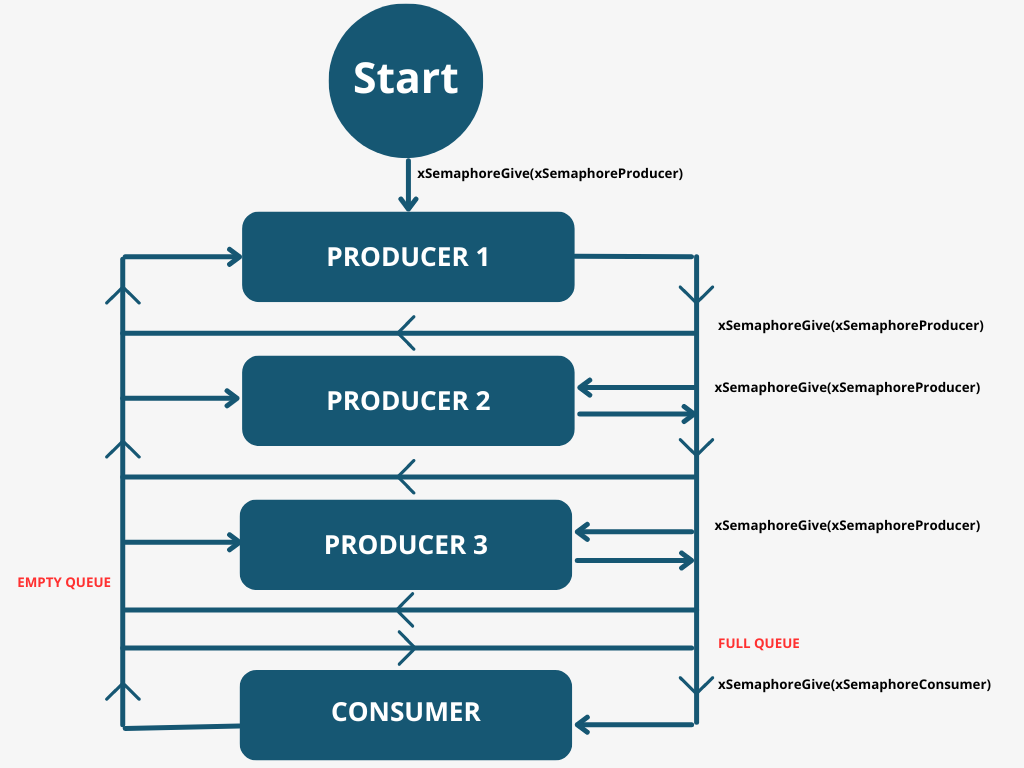
\includegraphics[width=0.5\textwidth]{img/precedence_diagram_semaphore1.png}
    \caption{Precedence Diagram - Semaphores (Example 1)}
    \label{fig:Precedence Diagram - Semaphores (Example 1)}
\end{figure}


\paragraph{Queue and Semaphores: Example 2}.
\label{par:Queue and Semaphores 2}
This demo application is a more advanced example which shows the usage of semaphores for tasks' synchronization.
The \texttt{main\_semaphore2} creates the \textbf{queue}, the \textbf{semaphores} and \textbf{four tasks} with the \textbf{SAME priority}:
\begin{itemize}
    \item three \textbf{PRODUCERS} which send items in the queue;
    \item one \textbf{CONSUMER} which reads from the queue.
\end{itemize}
Totally there are four \textbf{semaphores}:
\begin{itemize}
    \item three \textbf{binary semaphores} for the three \textbf{PRODUCERS};
    \item one \textbf{counting semaphore} for the \textbf{CONSUMER}.
\end{itemize}
Each \textbf{PRODUCER} inserts its value in the queue increasing the value of the counting semaphore of the \textbf{CONSUMER} (i.e, the value of \texttt{xSemaphoreConsumerCounting} represents the number of items currently available in the queue). Then it unblocks the next task as depicted in the following diagram:

\begin{figure}[H]
    \centering
    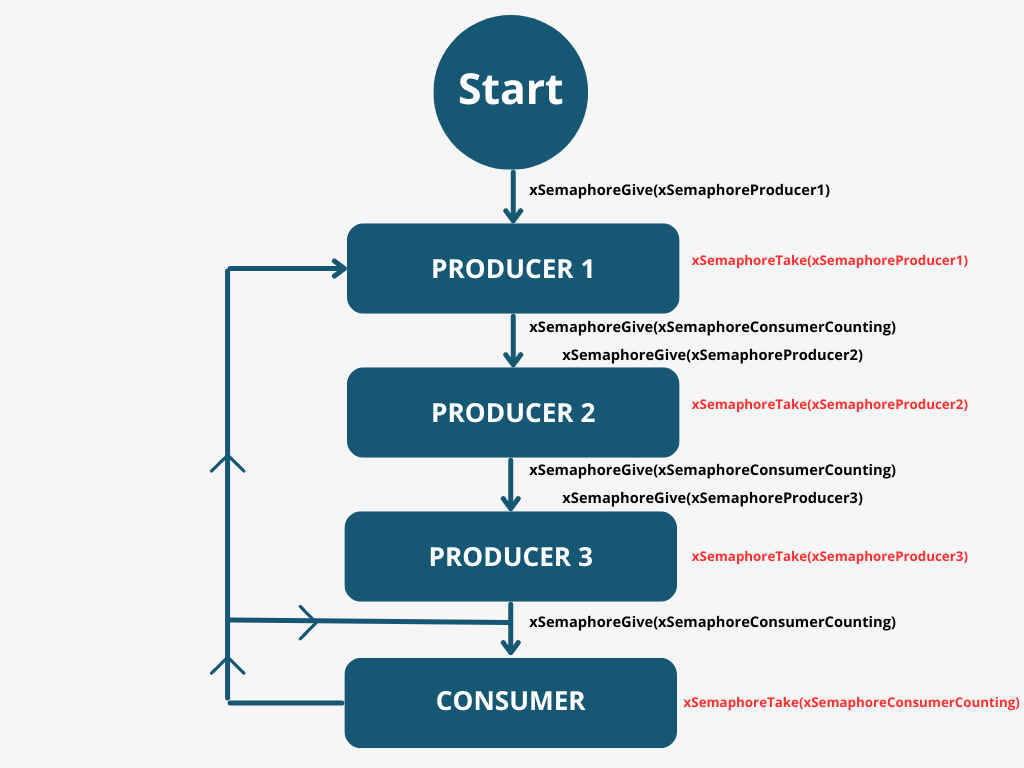
\includegraphics[width=0.5\textwidth]{img/precedence_diagram_semaphore2.png}
    \caption{Precedence Diagram - Semaphores (Example 2)}
    \label{fig:Precedence Diagram - Semaphores (Example 2)}
\end{figure}

Overall, each \textbf{PRODUCER} inserts its value and unblock the next task; then the \textbf{CONSUMER} reads out all the values previously inserted by the \textbf{PRODUCERS} before unblocking the \textbf{first PRODUCER} and the cycle continues indefinitely.
Again here the \textbf{priority} does not change the behaviour of the task.